\section{Propagación hacia adelante vectorizada (con matrices)}

 La sección anterior si bien nos da la idea somera de como van a ser las operaciones para el aprendizaje ahora veamos lo de forma matricial. Esto nos ayudará a en un momento dado escrbirlo en el lenguaje de nuestra convencia.
 
 
 Retomamando la red neuronal de la sección anterior ahora con pesos.
 
 \begin{figure}[H]
 \centering
 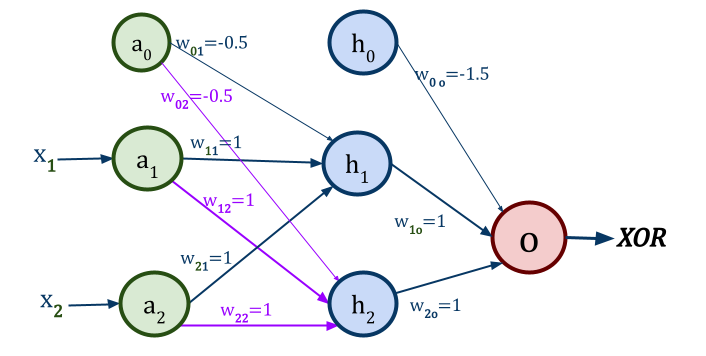
\includegraphics[scale=0.5]{../Figuras/XOR_pesos.png}
 \caption{Función XOR, con capa oculta}
 \label{fig:xorPesos}
\end{figure}

Ahora veamos a las entradas como un vector de la siguiente forma:
 $$
 A =
 \begin{bmatrix}
  a_{0}\\
  a_{1}\\
  a_{2}\\
 \end{bmatrix}
 =
 \begin{bmatrix}
  1\\
  0\\
  1\\
 \end{bmatrix}
 $$
 
 Ahora para poder hacer los siguientes cálculos acomodamos los pesos correspondientes a cada perceptron. Para el primer perceptron tomamos los pesos que están conectados desde la neurona de origen $a_{0}, a_{1}$ y $a_{2}$ hacia la neurona oculta $h_{1}$ (los indices de los pesos indican, el origen y el destino, en ese orden), los colocamos en un renglón de la matriz de pesos, así representamos nuestro primer perceptrón y hacemos lo mismo para $h_{2}$, así obtenemos la siguiente matriz de pesos:
 $$
 W =
 \begin{bmatrix}
  w_{01} & w_{11} & w_{21}  \\
  w_{02} & w_{12} & w_{22}\\
 \end{bmatrix}
 =
 \begin{bmatrix}
  -0.5 & 1 & 1\\
  1.5 & -1 & -1\\
 \end{bmatrix}
 $$
 
 Ya que tenemos la representación de las entradas y pesos en vactores podemos hacer la representación de la activación de estas neuronas de la capa oculta, que es de la forma $H = g(W * A)$, que de forma matricial lo podemos ecribir de la siguiente forma:
 $$
 H=
 \begin{bmatrix}
  h{1}  \\
  h{2}\\
 \end{bmatrix}
 = g \left(
 \begin{bmatrix}
  -0.5 & 1 & 1\\
  1.5 & -1 & -1\\
 \end{bmatrix}
 \begin{bmatrix}
  1 \\
  0 \\
  1 \\
 \end{bmatrix}
 \right) = g \left(
 \begin{bmatrix}
  0.5 \\
  0.5 \\
 \end{bmatrix}
\right) =
 \begin{bmatrix}
  1 \\
  1 \\
 \end{bmatrix}
$$
 
 La matriz resultante representa los valores de activación resultantes en cada perceptrón, el primer valor de la matriz representa el resultado de la activación de $h1$ y el segundo a $h2$. Así ahora tenemos al vector $H$ que sera el vector de entrada para la neurona de salida $o$, procedemos de la misma forma tomando en cuenta al sesgo $h_0$ y a los pesos en forma matricial, nos queda de la siguiente forma $o = g(W_{ho} * H)$:
 $$
 o =
 g \left(
 \begin{bmatrix}
  -1.5 & 1 & 1\\
 \end{bmatrix}
 \begin{bmatrix}
  1 \\
  1 \\
  1 \\
 \end{bmatrix}
 \right) = g \left(
 \begin{bmatrix}
  0.5 \\
 \end{bmatrix}
\right) =
 \begin{bmatrix}
  1 \\
 \end{bmatrix}
 $$
 
 
Hasta este momento ya logramos resolver la función XOR para una sola entrada, esta forma de resolver una red la llamaremos convención 1.
Si queremos que nos de la resupuesta a varias entradas al mismo tiempo tendríamos que modificar un poco la representación de nuestros valores, trasnpodiendo las matrices anteriores que teniamos. Que se verían de la siguiente forma:

 $$
 A^ {T} =
 \begin{bmatrix}
  a_{0} & a_{1} & a_{2}\\
 \end{bmatrix}
 =
 \begin{bmatrix}
  1 & 0 & 1 \\
 \end{bmatrix}
 $$

 $$
 W^ {T}  =
 \begin{bmatrix}
  w_{01} & w_{02}\\
  w_{11} & w_{12}\\
  w_{21} & w_{22}\\
 \end{bmatrix}
 =
 \begin{bmatrix}
  -0.5 & 1.5\\
  1 & -1\\
  1 & -1\\
 \end{bmatrix}
 $$

 $$
 H = g(A^{T}*W^{T}) \\
 $$

  $$
 H=
 \begin{bmatrix}
  h{1} & h{2}\\
 \end{bmatrix}
 = g \left(
 \begin{bmatrix}
  1 & 0 & 1\\
 \end{bmatrix}
 \begin{bmatrix}
  -0.5 & 1.5\\
  1 & -1\\
  1 & -1\\
 \end{bmatrix}
 \right) = g \left(
 \begin{bmatrix}
  0.5 &  0.5 \\
 \end{bmatrix}
\right) =
 \begin{bmatrix}
  1 &  1 \\
 \end{bmatrix}
$$

$$
 o =
 g \left(
 \begin{bmatrix}
  1 & 1 & 1\\
 \end{bmatrix}
 \begin{bmatrix}
  -1.5 \\
  1 \\
  1 \\
 \end{bmatrix}
 \right) = g \left(
 \begin{bmatrix}
  0.5 \\
 \end{bmatrix}
\right) =
 \begin{bmatrix}
  1 \\
 \end{bmatrix}
 $$
 
 
Esta forma se llama la convención 2, lo que estamos haciendo en la convención 2 es más bien poner nuestro ejemplar de manera horizontal. Así cada renglón de $A$ va a representar una entrada el primer valor de cada renglón siempre será el sesgo.
 Así al tener varias entradas de la siguiente forma:
 
 $$
 X =
 \begin{bmatrix}
  0 & 0 & 1 & 1\\
  0 & 1 & 0 & 1\\
 \end{bmatrix}
 $$
 
 A la matriz $A$ es $X$ transpuesta y le agregamos los sesgos, quedando así:
 $$
 A =
 \begin{bmatrix}
  1 & 0 & 0\\
  1 & 0 & 1\\
  1 & 1 & 0\\
  1 & 1 & 1\\
 \end{bmatrix}
 $$
 
 La capa oculta quedaría de la siguiente forma $H = g(W^{T}A)$

 $$
   H
 = g \left(
 \begin{bmatrix}
  1 & 0 & 0\\
  1 & 0 & 1\\
  1 & 1 & 0\\
  1 & 1 & 1\\
 \end{bmatrix} 
 \begin{bmatrix}
  -0.5 & 1.5\\
  1 & -1\\
  1 & -1\\
 \end{bmatrix}
 \right) = g \left(
 \begin{bmatrix}
  -0.5 &  1.5 \\
  0.5 &  0.5 \\
  0.5 &  0.5 \\
  1.5 &  -0.5 \\
 \end{bmatrix}
\right) =
 \begin{bmatrix}
  0 &  1 \\
  1 &  1 \\
  1 &  1 \\
  1 &  0 \\
 \end{bmatrix}
$$

 El resultado de esta matriz $H$ es que, la primera columna está representando la neurona que evalua la función OR y la segunda columna representa el NAND. Para obtener la salida de la neurona $o$ que es un AND, hariamos las mismas operaciones anteriores solo que con sus respectivos pesos y valores de $H^{T}$, así obteniendo lo siguiente $o = g(H^{'}W^{T}) = XOR$:
 
 $$
 o =
 g \left(
 \begin{bmatrix}
  1 & 0 & 1 \\
  1 & 1 & 1 \\
  1 & 1 & 1 \\ 
  1 & 1 & 0\\
  \end{bmatrix}
 \begin{bmatrix}
  -1.5 \\
  1 \\
  1 \\
 \end{bmatrix}
  \right) = g \left(
 \begin{bmatrix}
  -0.5 \\
  0.5 \\
  0.5 \\
  -0.5 \\
 \end{bmatrix}
\right) =
 \begin{bmatrix}
  0 \\
  1 \\
  1 \\
  0 \\
 \end{bmatrix}
 $$


Más adelante esta representación, nos ayudará cuando estemos trabajando con redes neuronales que necesiten \emph{diferentes tipos de características}, como; edades, número de hijos, tamaño de una casa, etc. 
 Esta anotación es mucho más visual para la forma en que vamos a recibir la información (tabla de datos), por eso es más usada está versión.

